\documentclass[a4paper,10pt]{article}
\usepackage[french]{babel} 
\usepackage[utf8x]{inputenc}
\usepackage[T1]{fontenc}
\usepackage{lmodern}
\usepackage{makeidx}
\usepackage{multicol}
\usepackage{hyperref}
\usepackage{pdfpages}

\newcommand{\etal}{\textit{et al.}}

\title{
  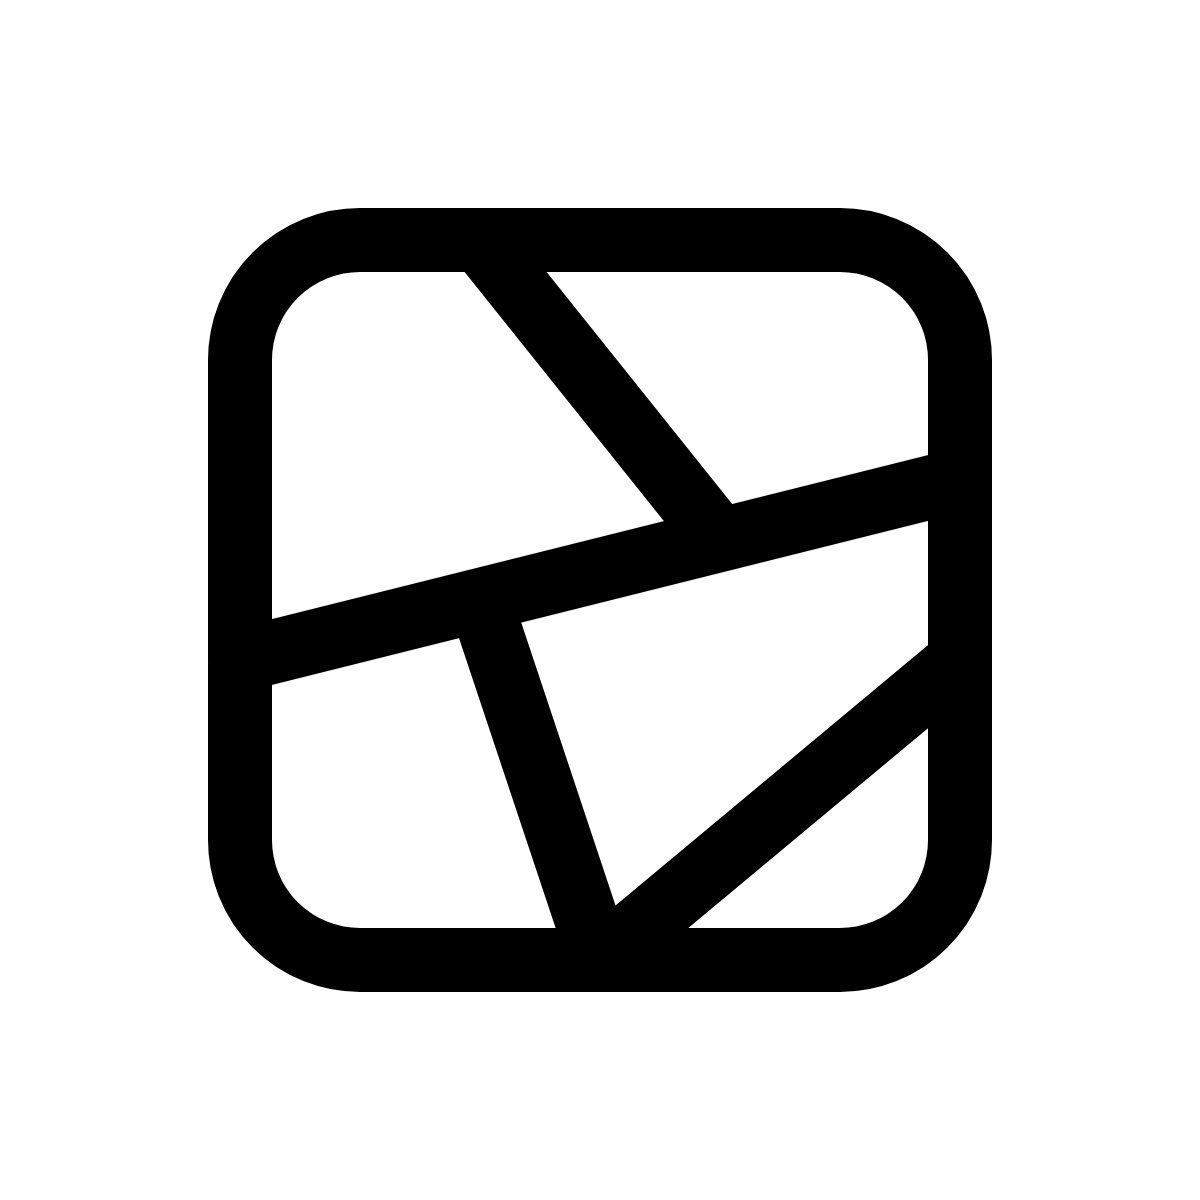
\includegraphics[width=2cm]{../iconography/phragment-black.png}\\
  \bsc{Phragment}\\
  \large{
    Une tentative protocole pour des conversations décentralisées
    où tout le monde est propriétaire de son contenu\\~\\~\\
    \textbf{version} \texttt{0.0.1}
  }
}

\date{}
\author{
  Xavier \bsc{Van de Woestyne}\\
  \texttt{xaviervdw@gmail.com}\\
  \small{https://xvw.github.io}
}


\hypersetup{ hidelinks, }
\addto{\captionsfrench}{\renewcommand{\abstractname}{}}

\begin{document}

\maketitle

\begin{abstract}
  A l'heure ou le web décentralisé revient à la tendance, pour de multiples
  raisons valables (écologiques, morales et idéologiques, ouvertures de
  perspectives), on trouve beaucoup de solutions qui pallient à des soucis
  liés à l'excès de centralisation dans le web. \bsc{Phragment} est un
  protocole dont l'objectif initial est de servir un système de commentaires
  pour une application web statique, tâchant de permettre aux intervenants
  de contrôler leurs différents contenus. Le protocole ne décrit aucune
  innovations particulières et souffre d'un manque d'ergonomie flagrant,
  cependant, j'assume parfaitement le plaisir de réinventer, encore une fois,
  une roue, bancale et peu robust. L'objectif de ce document est de survoler
  les motivations (et le contexte) d'un tel protocol, son formalisme,
  l'élaboration d'un client de référence, le survol de certains cas d'usages,
  les améliorations possibles, points de blocages et faiblesses intrinsèques.
  \\~\\
  Ce document est assez informel, il repose avant tout sur un besoin
  personnel, et est rédigé dans un style bien peu générique. Pour tout lecteurs
  potentiels, prenez donc ce document comme une feuille de route, rédigée
  au long de l'implémentation du protocole et de ses cas d'usages.
  \\
\end{abstract}

% \section*{Dans le monde des sites statiques}

En tant que développeur, l'utilisation d'un système de génération de page en
amont apporte généralement plusieurs bienfaits, par exemple, la génération
des pages ne reposant sur aucune mécanique dynamique exposée au client,
on diminue la maintenance sécuritaire de cette application web.
Pour ma part, les avantages majeurs de cette approche est que je peux très
facilement héberger ma page personnelle sur des hébergeurs qui ne servent
que des fichiers statiques, et je suis assez libre des technologies que je
peux utiliser pour construire ma page, en amont, libéré de toute contraintes
d'hébergement. De plus, le flot de développement et de publication est
généralement très commode pour un développeur. On peut rédiger dans son
éditeur favoris, utilisant un format de \textit{markup} libre et rendant le
versionnement du code et de l'application assez simplement via des
gestionnaires de versions classiques, avec une séparation claire entre la
structure du document et son contenu.
\\~\\
Cependant, l'absence de mécanique dynamique restreint le champ des possibles.
Il est, par exemple, bien plus complexe de mettre en place de l'interactivité
partagée avec les utilisateurs de l'application. Dès lors que l'on construit
un blog, la mise en place de commentaires sur les publications implique
plus de travail. On pourrait résumer les opportunités d'interactivité en
trois méthodes : \\
\begin{itemize}
\item implantation d'un minimum dynamique ;
\item utilisation d'un tiers ;
\item invitation à la participation sur le code directement.
\end{itemize}

\subsection*{L'interaction au moyen de tiers}

\newpage
\bibliographystyle{unsrt}
\bibliography{phragment.bib}

\end{document}
